\section{Parallel Architectures}

\subsection{Flynn's Taxonomy}

\subsubsection{Instruction Level}
\begin{itemize}
    \item Single Instruction (SI) - System in which all processors execute the same instruction
    \item Multiple Instruction (MI) - System in which different processors execute may execute different instructions
\end{itemize}

\subsubsection{Data Level}
\begin{itemize}
    \item Single Data (SD) - System in which all processors operate on the same data
    \item Multiple Data (MD) - System in which different processors may operate on different data
\end{itemize}

\subsubsection{Existing Architectures}

\begin{figure}[h]
    \centering
    \begin{tabular}{c | c | c}
           & SD   & MD   \\
        \hline
        SI & SISD & SIMD \\
        \hline
        MI & MISD & MIMD \\
    \end{tabular}
    \caption{Possible processor architectures. MISD is the exception.}
    \label{fig:flynn}
\end{figure}

\paragraph{SISD}
The classic Von Neumann architecture, present in serial processors
\begin{figure}[h]
    \centering
    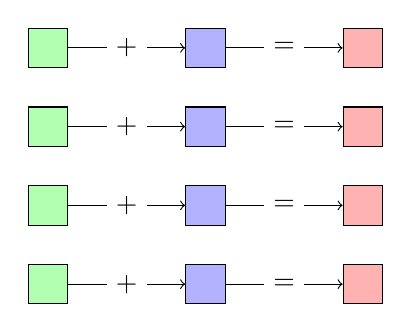
\begin{tikzpicture}

        \foreach \y in {0,..., 3}
            {
                \node[name=1_\y, draw, rectangle, minimum size=0.5cm, fill=green!30] at (0, \y) {};
                \node[name=2_\y, draw, rectangle, minimum size=0.5cm, fill=blue!30] at (2, \y) {};
                \node[name=3_\y, draw, rectangle, minimum size=0.5cm, fill=red!30] at (4, \y) {};
                \draw[->] (1_\y) -- node [fill=white] {$+$} (2_\y);
                \draw[->] (2_\y) -- node [fill=white] {$=$} (3_\y);
            }
    \end{tikzpicture}
    \caption{SISD Processing Example. One instruction is applied to each data item.}
    \label{}
\end{figure}

\paragraph{SIMD}
The data is divided among the processors and each item is subjected to the same sequence of instructions. Present in modern CPUs through Advanced Vector Extensions (AVX), as well as GPUs.
\begin{figure}[h]
    \centering
    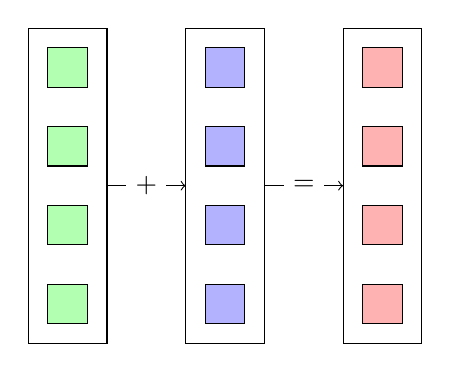
\begin{tikzpicture}

        \foreach \y in {0,..., 3}
            {
                \node[name=1_\y, draw, rectangle, minimum size=0.5cm, fill=green!30] at (0, \y) {};
                \node[name=2_\y, draw, rectangle, minimum size=0.5cm, fill=blue!30] at (2, \y) {};
                \node[name=3_\y, draw, rectangle, minimum size=0.5cm, fill=red!30] at (4, \y) {};
            }
        \draw (-.5, -.5) rectangle (.5, 3.5);
        \draw (1.5, -.5) rectangle (2.5, 3.5);
        \draw (3.5, -.5) rectangle (4.5, 3.5);
        \draw[->] (.5, 1.5) --  node[fill=white] {$+$} (1.5, 1.5);
        \draw[->] (2.5, 1.5) -- node[fill=white] {$=$} (3.5, 1.5);
    \end{tikzpicture}
    \caption{SIMD Processing Example. One instruction is applied to a block of data items.}
    \label{}
\end{figure}

\paragraph{MISD}
Possible to envision as a pipeline at most, since it is not possible for multiple instructions to execute at the same time over the same data item.

\paragraph{MIMD}
Collection of autonomous processors executing independent programs, such as a distributed network or cluster.
MIMD architectures can be categorized under four designations, each with different purposes, some of these architectures may be composed to form more complex systems.

\begin{figure}[h]
    \centering
    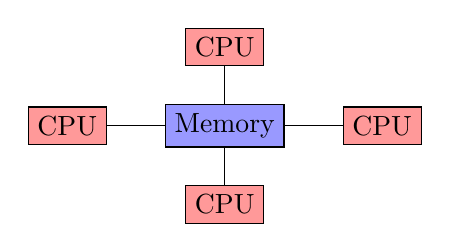
\begin{tikzpicture}
        % \draw (0, 0) grid (4,2);
        \node[draw, fill=blue!40, name=memory] at (2, 1) {Memory};
        \node[draw, fill=red!40, name=cpu_1] at (0, 1) {CPU};
        \node[draw, fill=red!40, name=cpu_2] at (2, 2) {CPU};
        \node[draw, fill=red!40, name=cpu_3] at (2, 0) {CPU};
        \node[draw, fill=red!40, name=cpu_4] at (4, 1) {CPU};
        \draw[-] (cpu_1) -- (memory);
        \draw[-] (cpu_2) -- (memory);
        \draw[-] (cpu_3) -- (memory);
        \draw[-] (cpu_4) -- (memory);
    \end{tikzpicture}
    \caption{Uniform Memory Access (UMA). This architecture suffers from the need of synchronization among memory accesses. We can picture this as several CPUs accessing common RAM.}
    \label{fig:sm:uma}
\end{figure}

% \begin{figure}[h]
%     \centering
%     \begin{tikzpicture}
%         \draw (-5, -2) grid (5, 2);
%         \draw (-4.5, .5) rectangle (-.5, 1.5);
%         \draw [-] (-2.5, .5) -- (-2.5, 1.5);
%     \end{tikzpicture}
%     \caption{Non-Uniform Memory Access (NUMA). Common in distributed architectures.}
%     \label{fig:sm:numa}
% \end{figure}

\subsection{Software Taxonomies}

Applying Flynn's taxonomy to software we observe the following patterns.

\begin{itemize}
    \item Data Parallel (SIMD) - Parallelism that is a result of identical operations applied concurrently on different data items. This approach is difficult to apply to complex problems.
    \item Single Program, Multiple Data (SPMD) - A single program is run across multiple processing units (computers, processors, threads). Processing units execute the same code but do not work in lock-step.
\end{itemize}

\subsection{Memory}

Memory can be split into shared memory or distributed memory.

\subsubsection{Shared Memory}

Shared memory represents a global memory space, it is accessed by every processor.
Each processor has a local cache (L1, L2, L3) which keep portions of the memory for faster access.
The L1 and L2 caches are available at a core level while the L3 cache is shared among cores.

Shared memory is easier to program with, several frameworks are available (e.g. OpenMP, OpenACC).
Low latency for data sharing between tasks.
However the programmer is responsible for synchronization, furthermore the memory access is non-uniform (NUMA) and accesses to global memory (RAM) can be a bottleneck.

\subsubsection{Distributed Memory}

Memory is shared between processes using messages (OpenMPI), this allows to exploit distributed computing architectures in a cost effective way.

Memory scales based on the number of processors and the access to local memory is fast.

This approach however is complex due to difficulties in programming communication effectively and data structures may be difficult to distribute.